\chapter{Neural network}\label{chap:nn}

\section{Neural network architecture}

Given the nature of the data, we decided to use a neural network to predict the
changes in the body shape. Since the data is temporal, we need to use a neural
network architecture that can handle temporal data.

There are different neural network architectures that work well with temporal
data. Recurrent neural networks are a type of neural networks that feed the
output of the previous step as input to the next step. This allows them to
remember information from previous steps, which is useful for time series.
However, they can `forget' information from the beginning of the sequence,
which is a problem known as vanishing gradients. There are some variations of
recurrent neural networks that try to solve this problem, such as \gls{lstm}
and \gls{gru}.

Transformer networks are a relatively new type of neural network that has been
used with great success in natural language processing. They are based on
attention mechanisms, which allow them to focus on specific parts of the input
sequence. This makes them very useful for time series, since they can focus on
the most relevant parts of the sequence. The big disadvantage of transformer
networks for this application is that they require large amounts of training
data\todo[]{citation needed}, which is not available in this case.

We ended up using an neural network architecture that uses an \gls{lstm}.

\section{Neural network architecture}

We used the PyTorch library to implement our custom neural network
architecture.

\begin{figure}
    \centering
    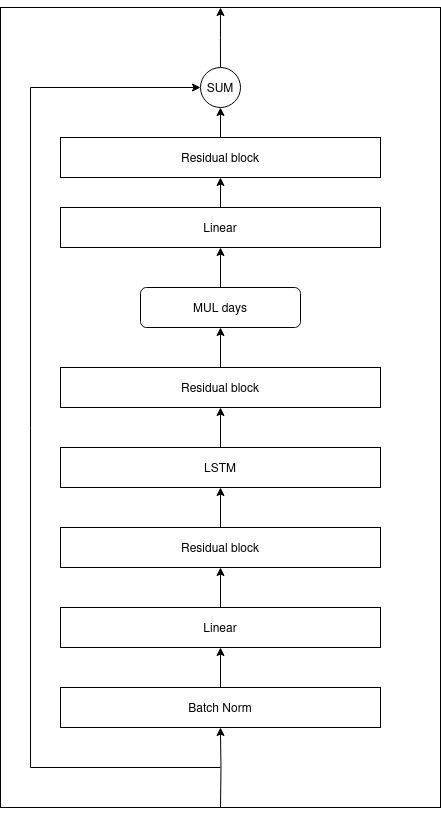
\includegraphics[width=8cm]{files/nn_diagram}
    \caption{Diagram of the neural network architecture}
\end{figure}

To solve the problem of having patient's with different numbers of sessions, we
used PyTorch's \texttt{pack\_padded\_sequence} and
\texttt{pad\_packed\_sequence}, which allow us to pack the sequences into a
single tensor, and then unpack them afterwards. With another tensor of
\textit{lengths}, we can then use the packed sequences as input to the neural
network, and the \gls{lstm} will ignore the values after the length of the
sequence.

\subsection{Variability in the dates of the sessions}

The dataset's sessions are not uniformly spaced in time, varying from a few
days to several months apart. This is a problem for neural networks, since they
work best with uniformly spaced data. To solve this problem, we decided to make
the neural network predict the daily change instead.

This was accomplished by adding a residual connection between the input and the
output of the neural network, and multiplying the output by the number of days
until the next session. This way, the neural network can learn to predict the
daily change, and the output is scaled to the number of days until the next
session.

\section{Training}

The neural network inputs a tensor of shape (batch size, max sequence length,
number of features), a tensor of shape (batch size, 1) containing the length of
the current sequence, and a scalar representing the number of days until the
next session. It returns a tensor of shape (batch size, max sequence length,
number of features) containing the predicted values for the next session.

\begin{itemize}
    \item The neural network takes as input:
          \begin{itemize}
              \item A tensor of shape (batch size, max sequence length, number of features).
              \item A tensor of shape (batch size, 1) containing the length of the current
                    sequence.
              \item A scalar representing the number of days until the next session.
          \end{itemize}
    \item The neural network returns:
          \begin{itemize}
              \item A tensor of shape (batch size, max sequence length, number of features) that
                    contains the predicted values for the next session.
          \end{itemize}
\end{itemize}

For features, we concatenate the \gls{smpl} parameters shape ($\beta$) with the
patient's height, weight, and age. We also experimented with using body fat
percentage and muscle mass percentage, but the results didn't improve. We used
the AdamW optimizer with a variable learning rate and weight decay, and MSE
loss.

\section{Results}

We will delve into the results in more detail in the next chapter, but we will
show some examples of our model's predictions here.

\begin{figure}[h]
    \centering
    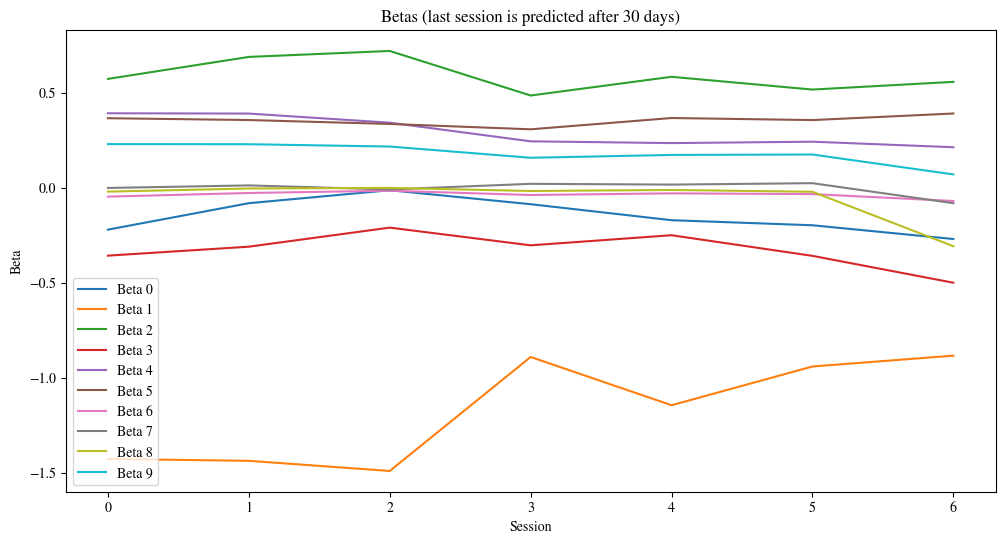
\includegraphics[width=\textwidth]{files/predicted_betas}
    \caption{Shape parameters for a patient and the model's prediction.}
\end{figure}

\begin{figure}[h]
    \centering
    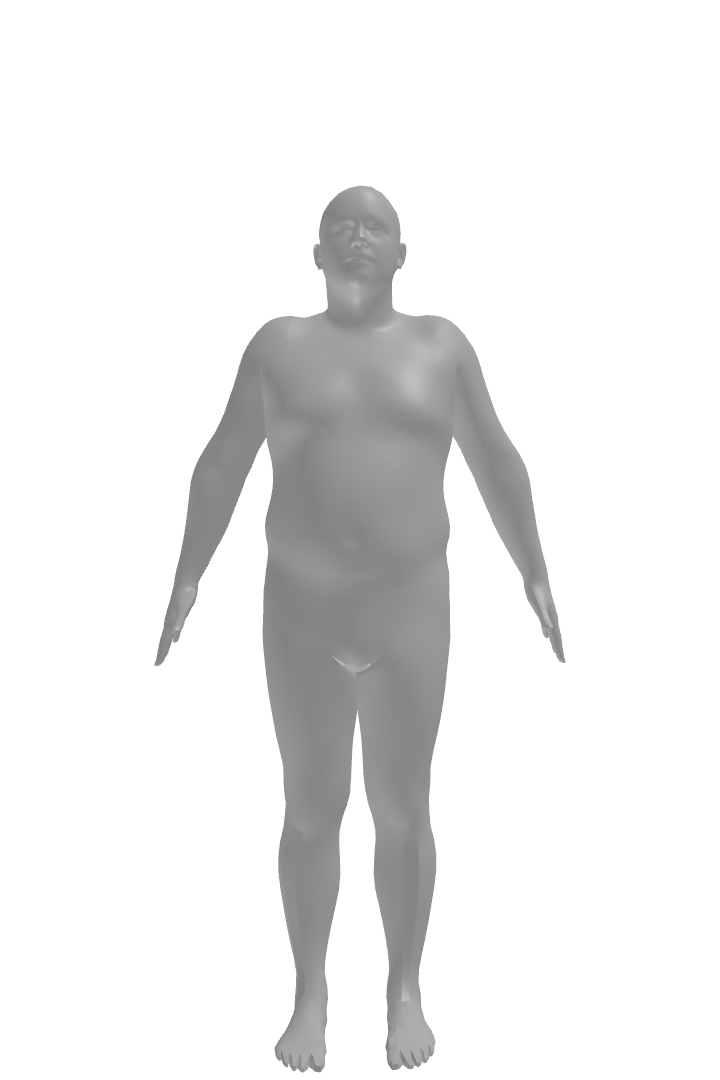
\includegraphics[width=120pt]{files/patient_2/2_6}
    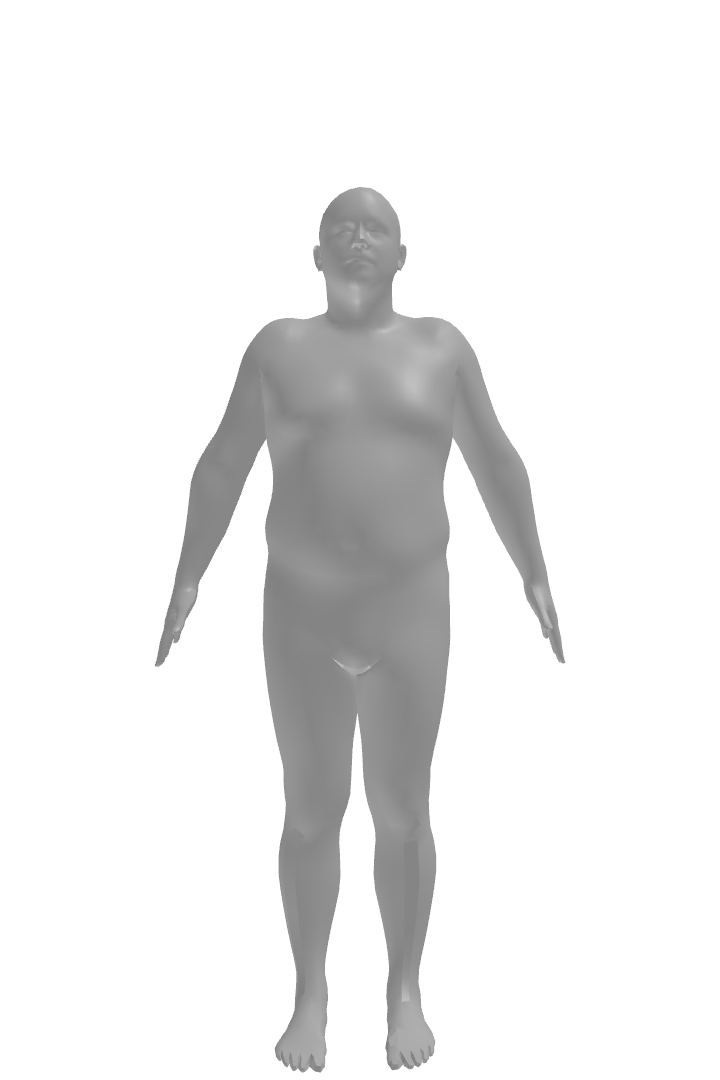
\includegraphics[width=120pt]{files/patient_2/2_7}
    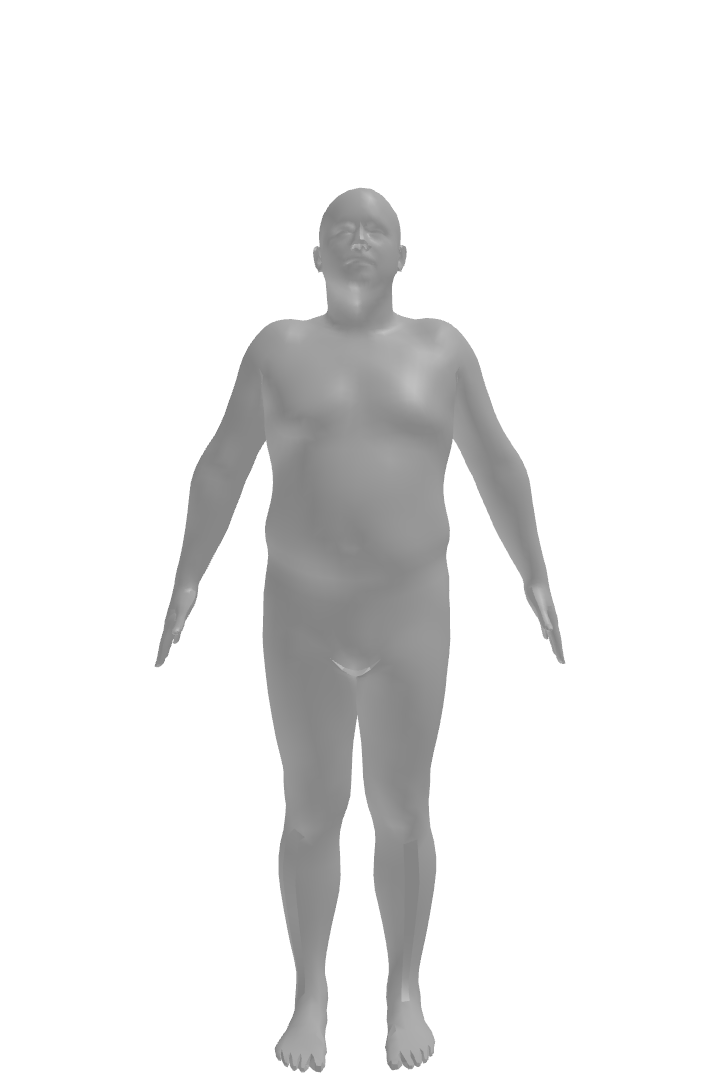
\includegraphics[width=120pt]{files/patient_2/2_8}
    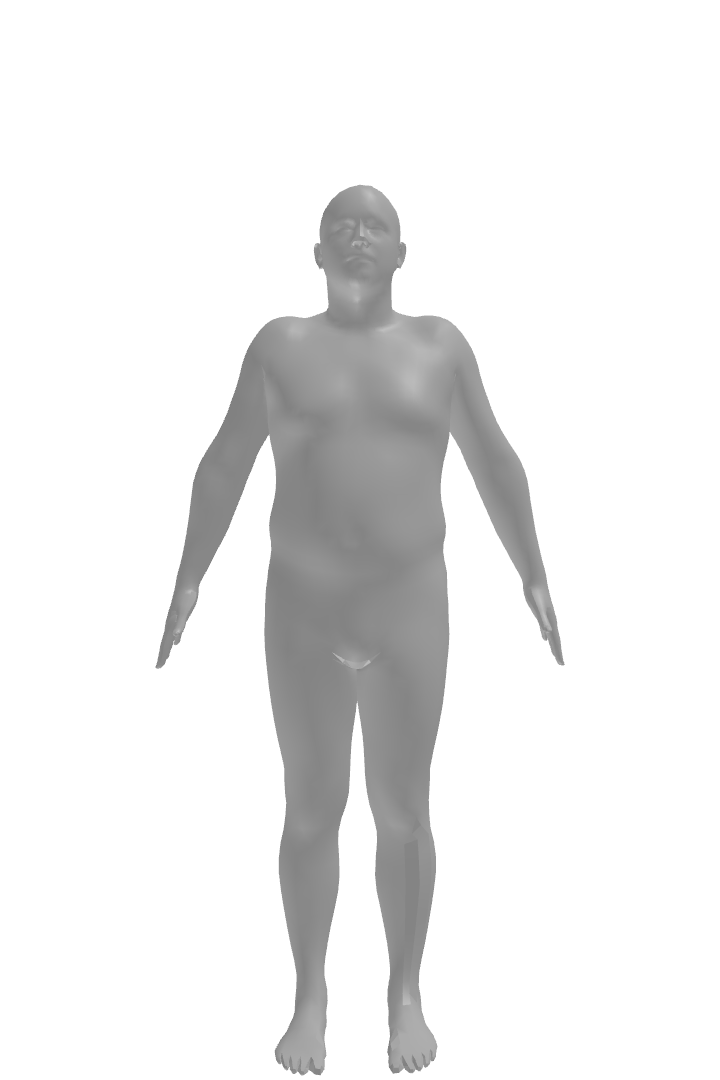
\includegraphics[width=120pt]{files/patient_2/2_9}
    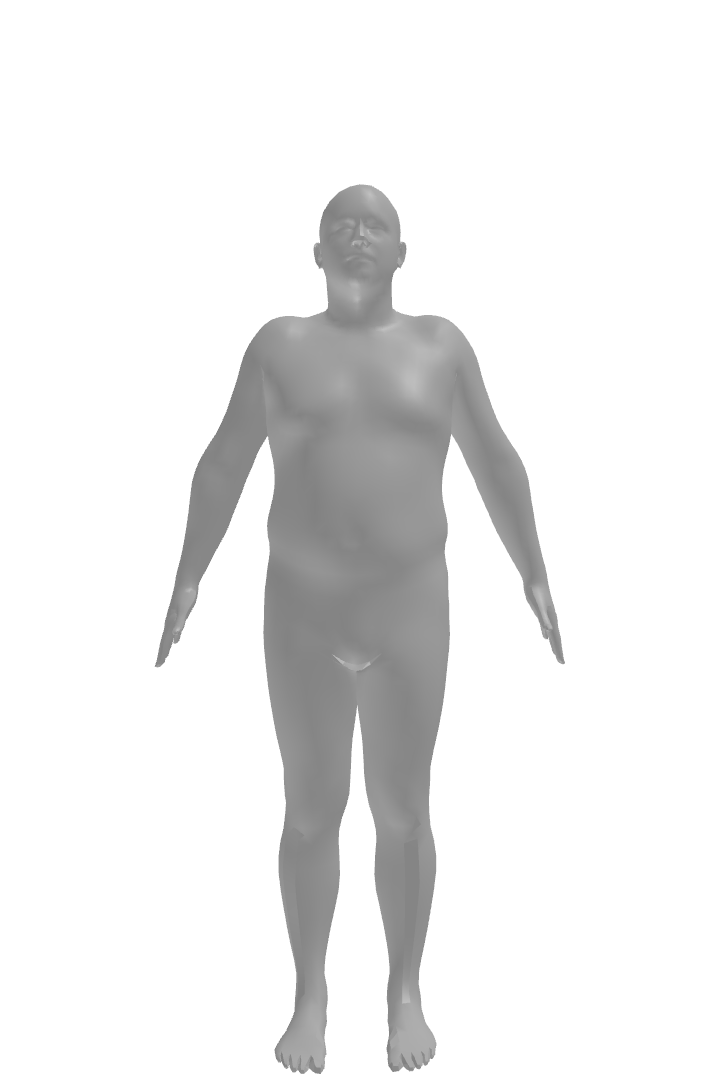
\includegraphics[width=120pt]{files/patient_2/2_10}
    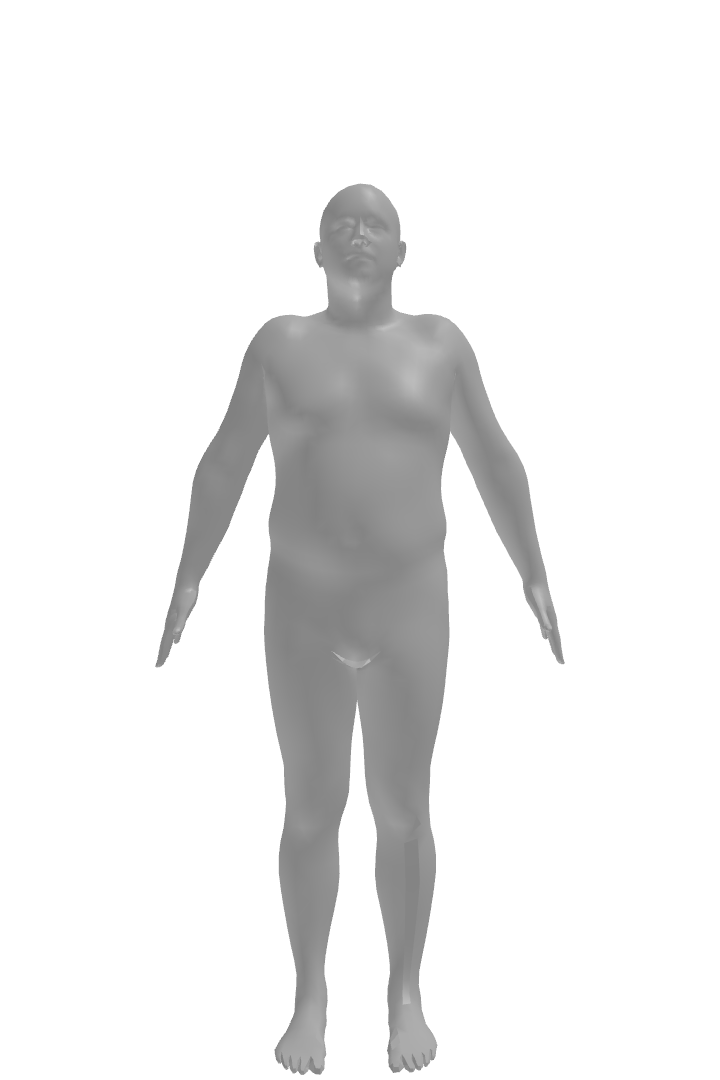
\includegraphics[width=120pt]{files/patient_2/2_11}
    \linebreak
    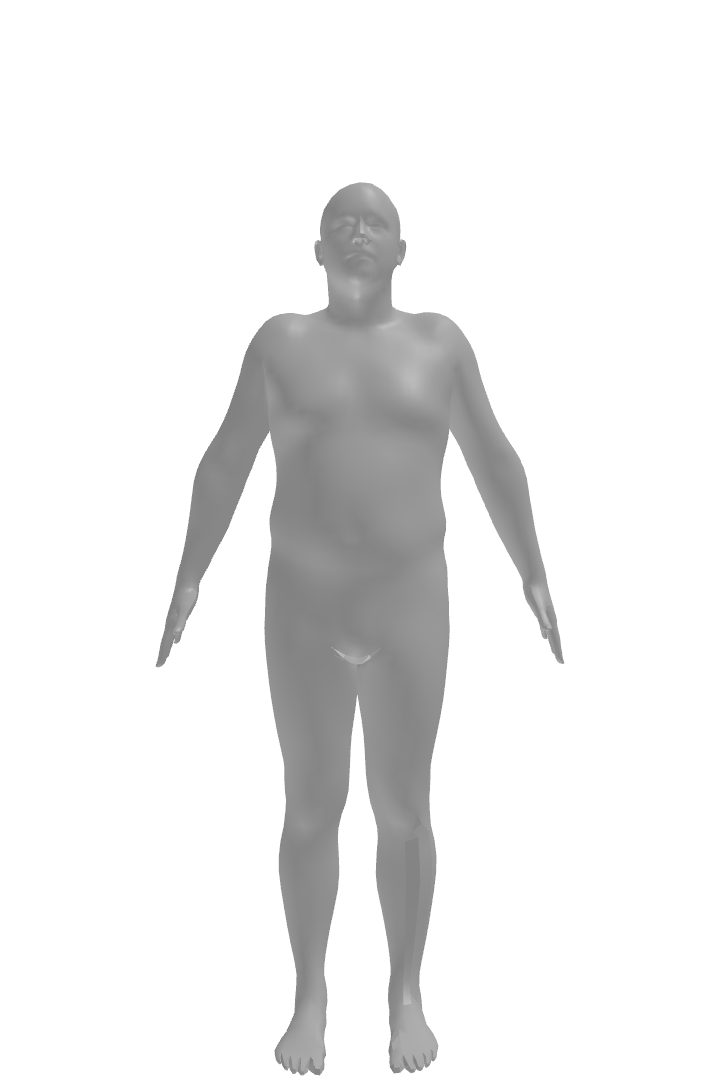
\includegraphics[width=120pt]{files/patient_2/2_predicted}
    \caption[Reconstructed 3D model of the patient's body]{Reconstructed 3D
        model of the patient's body. The last image is the model's prediction after a month of
        the last session. There are a total of 74 days between the first and last session.}
\end{figure}
